\documentclass[a4paper]{scrartcl}

\usepackage[
    fancytheorems, 
    fancyproofs, 
    noindent, 
]{adam}

\usepackage{physics}
\usepackage{amsmath}
\usepackage{tikz}
\usepackage{mathdots}
\usepackage{yhmath}
\usepackage{cancel}
\usepackage{color}
\usepackage{siunitx}
\usepackage{array}
\usepackage{multirow}
\usepackage{amssymb}
\usepackage{gensymb}
\usepackage{tabularx}
\usepackage{extarrows}
\usepackage{booktabs}
\usetikzlibrary{fadings}
\usetikzlibrary{patterns}
\usetikzlibrary{shadows.blur}
\usetikzlibrary{shapes}


\title{Analysis and Topology}
\author{Adam Kelly (\texttt{ak2316@cam.ac.uk})}
\date{\today}

\allowdisplaybreaks

\begin{document}

\maketitle

This course is a second course in Analysis and a first course in Topology. 
We will study both concrete results over $\R$ and $\C$ concerning uniform convergence and continuity, and we will also move to more abstract settings to discuss metric and topological spaces, completeness, connectedness and compactness.

This article constitutes my notes for the `Analysis and Topology' course, held in Michaelmas 2021 at Cambridge. These notes are \emph{not a transcription of the lectures}, and differ significantly in quite a few areas. Still, all lectured material should be covered.



\tableofcontents

% \section{Introduction}

% \subsection{Outline of the Course}

% This is a second course in Analysis and a first course in Topology. 

% \begin{enumerate}
%     \item Uniform convergence and uniform continuity
%     \item Metric spaces
%     \item Completeness and the contraction mapping theorem
%     \item Topological spaces
%     \item Connectedness
%     \item Compactness
%     \item Differentiation and the inverse function theorem
% \end{enumerate}

% \subsection{Prerequisites}

% Of course the Analysis I course from Part IA is going to assumed knowledge.

% \subsection{Books}

% Burkill \& Burkill and Sutherland are both good. Sutherland has a good motivation about abstraction.

% \subsection{Example Sheets}

% Plus questions are not exam questions.

\section{Uniform Convergence and Uniform Continuity} 

\subsection{Uniform Convergence}
Recall the notion of convergence for a sequence in $\R$ or $\C$:

\begin{definition}[Convergence of a Sequence]
    A sequence $a_{1}, a_{2}, \cdots \in \mathbb{R}$ is said to \vocab{converge} to the limit $a$ if given any $\epsilon>0$, we can find an integer $N$ such that $\left|a_{n}-a\right|<\epsilon$ for all $n \geq N$. We write $a_{n} \rightarrow a$ as $n \rightarrow \infty$
\end{definition}

That is, given any $\varepsilon$, there is some point in the sequence after which the terms of the sequence are $\varepsilon$ close to $a$. 

Our aim is going to define a similar notion to make sense of $f_n \rightarrow f$, where $f_n$ is a sequence of functions.

\begin{definition}[Uniform Convergence]
    A sequence of functions $f_1, f_2, \dots$ with $f_i : S \rightarrow \R$ is said to \vocab{converge uniformly} on $S$ to a function $f:S \rightarrow \R$ if given any $\varepsilon > 0$, we can find an integer $N$ such that $|f_n(x) - f(x)| < \varepsilon$, for any $x \in S$.
\end{definition}

\begin{remark}
    In the above definition, our $N$ can depend only on $\varepsilon$, and must be independent of the particular choice of $x \in S$. This is why we call this \emph{uniform} convergence -- because the property has to hold uniformly across the domain. 
\end{remark}

\begin{center}
    


    \tikzset{every picture/.style={line width=0.75pt}} %set default line width to 0.75pt        

    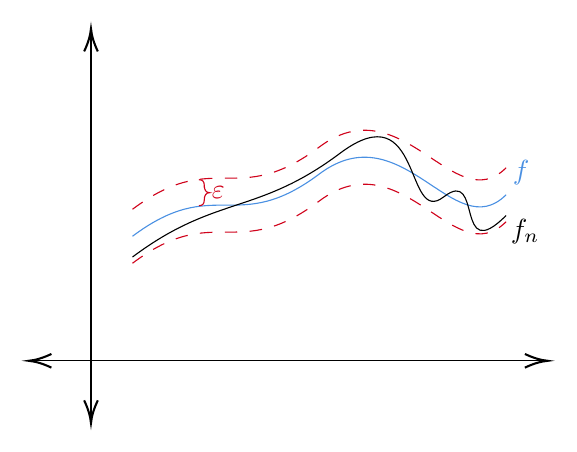
\begin{tikzpicture}[x=0.75pt,y=0.75pt,yscale=-1,xscale=1]
    %uncomment if require: \path (0,300); %set diagram left start at 0, and has height of 300
    
    %Straight Lines [id:da15070589522945865] 
    \draw    (120,42) -- (120,228) ;
    \draw [shift={(120,230)}, rotate = 270] [color={rgb, 255:red, 0; green, 0; blue, 0 }  ][line width=0.75]    (10.93,-3.29) .. controls (6.95,-1.4) and (3.31,-0.3) .. (0,0) .. controls (3.31,0.3) and (6.95,1.4) .. (10.93,3.29)   ;
    \draw [shift={(120,40)}, rotate = 90] [color={rgb, 255:red, 0; green, 0; blue, 0 }  ][line width=0.75]    (10.93,-3.29) .. controls (6.95,-1.4) and (3.31,-0.3) .. (0,0) .. controls (3.31,0.3) and (6.95,1.4) .. (10.93,3.29)   ;
    %Straight Lines [id:da06812433005878815] 
    \draw    (338,200) -- (92,200) ;
    \draw [shift={(90,200)}, rotate = 360] [color={rgb, 255:red, 0; green, 0; blue, 0 }  ][line width=0.75]    (10.93,-3.29) .. controls (6.95,-1.4) and (3.31,-0.3) .. (0,0) .. controls (3.31,0.3) and (6.95,1.4) .. (10.93,3.29)   ;
    \draw [shift={(340,200)}, rotate = 180] [color={rgb, 255:red, 0; green, 0; blue, 0 }  ][line width=0.75]    (10.93,-3.29) .. controls (6.95,-1.4) and (3.31,-0.3) .. (0,0) .. controls (3.31,0.3) and (6.95,1.4) .. (10.93,3.29)   ;
    %Curve Lines [id:da9975807479144934] 
    \draw [color={rgb, 255:red, 74; green, 144; blue, 226 }  ,draw opacity=1 ]   (140,140) .. controls (180,110) and (190,140) .. (230,110) .. controls (270,80) and (295,145) .. (320,120) ;
    %Curve Lines [id:da8386196196350342] 
    \draw [color={rgb, 255:red, 208; green, 2; blue, 27 }  ,draw opacity=1 ] [dash pattern={on 4.5pt off 4.5pt}]  (140,127) .. controls (180,97) and (190,127) .. (230,97) .. controls (270,67) and (295,132) .. (320,107) ;
    %Curve Lines [id:da7136000427009845] 
    \draw [color={rgb, 255:red, 208; green, 2; blue, 27 }  ,draw opacity=1 ] [dash pattern={on 4.5pt off 4.5pt}]  (140,153) .. controls (180,123) and (190,153) .. (230,123) .. controls (270,93) and (295,158) .. (320,133) ;
    %Shape: Brace [id:dp021850826872210183] 
    \draw  [color={rgb, 255:red, 208; green, 2; blue, 27 }  ,draw opacity=1 ] (172,125.25) .. controls (173.71,125.25) and (174.57,124.39) .. (174.57,122.68) -- (174.57,122.68) .. controls (174.57,120.23) and (175.43,119) .. (177.15,119) .. controls (175.43,119) and (174.57,117.77) .. (174.57,115.32)(174.57,116.43) -- (174.57,115.32) .. controls (174.57,113.61) and (173.71,112.75) .. (172,112.75) ;
    %Curve Lines [id:da39763918210258864] 
    \draw    (140,150) .. controls (180,120) and (200,130) .. (240,100) .. controls (280,70) and (271,135.75) .. (290,121) .. controls (309,106.25) and (295,155) .. (320,130) ;
    
    % Text Node
    \draw (177,119) node [anchor=west] [inner sep=0.75pt]  [color={rgb, 255:red, 208; green, 2; blue, 27 }  ,opacity=1 ]  {$\varepsilon $};
    % Text Node
    \draw (322,116.6) node [anchor=south west] [inner sep=0.75pt]  [color={rgb, 255:red, 74; green, 144; blue, 226 }  ,opacity=1 ]  {$f$};
    % Text Node
    \draw (321,130.4) node [anchor=north west][inner sep=0.75pt]  [color={rgb, 255:red, 0; green, 0; blue, 0 }  ,opacity=1 ]  {$f_{n}$};
    
    
    \end{tikzpicture}
    

\end{center}


Equivalently, we could say that for all $\varepsilon > 0$ there's some $N \in \N$ such that for all $n \geq N$ we have $\sup_{x \in S} |f_n(x) - f(x)| < \varepsilon$.

The above definition implies that if we fix some value of $x$ that $f_1(x), f_2(x), \dots$ converges to $f(x)$. This implies that the function $f$ is unique, due to the uniqueness of limits in $\R$ and $\C$. We sometimes call $f$ the \vocab{uniform limit}.

\begin{definition}[Pointwise Convergence]
We say that $f_n$ \vocab{converges pointwise} on $S$ to $f$ if $f_n(x) \rightarrow f(x)$ for every $x \in S$.
\end{definition}
\begin{remark}
    In this definition our `$N$' can depend on $\varepsilon$ \emph{and} $x$! This makes it a much weaker notion than uniform convergence, and clearly uniform convergence implies pointwise convergence.
\end{remark}

\begin{example}[Checking Uniform Convergence]
    Consider the sequence of functions $f_n(x) = x^2 \cdot e^{-n x}$ for $n \in \N$ and $x \in \R^+$. We want to know if this sequence of functions converges uniformly on this domain.

    Since pointwise convergence is implied by uniform convergence, we can first check the pointwise limit exists and use that to specify $f$ in our definition of uniform convergence.

    Fix $x \geq 0$. Then $x^2 e^{-nx} \rightarrow 0$ as $n \rightarrow 0$. So $f_n$ tends to $0$ (the zero function) pointwise on $\R^+$. We can now check if $f_n$ converges uniformly to the zero function.

    We can attempt to compute the quantity
    $$
    \sup_{x \geq 0} |f_n(x) - 0| =  \sup_{x \geq 0} f_n(x).
    $$
    One approach would be to differentiate it, which would need some care. A better way is to find an upper bound on $|f_n(x) - f(x)|$ which does not depend on $x$. In this case we can bound
    $$
    0 \leq x^2 e^{-nx} = \frac{x^2}{1 + nx + n^2x^2/2 + \cdots} \leq \frac{2}{n^2},
    $$
    for all $x \geq 0$. Thus $\sup_{x \geq 0} f_n(x) \leq 2/n^2 \rightarrow 0$ as $n \rightarrow \infty$. So does indeed $f_n \rightarrow 0$ uniformly on $\R^+$.
\end{example}

\begin{example}[Showing Uniform Convergence Doesn't Hold]
    Consider the sequence of functions $f_n(x) = x^n$ for $n \in \N$, over the domain $[0, 1]$.

    We can compute the limit as
    $$
    x^n \rightarrow f(x) = \begin{cases}
        0 &\mbox{if } 0 \leq x < 1, \\
        1 &\mbox{if } x = 1.
       \end{cases}
    $$
    This implies that $\sup_{x \in [0, 1]} |f_n(x) - f(x)| = 1$. So this doesn't tend to zero, and thus the sequence of functions $f_n$ converges pointwise but not uniformly.

    Alternatively, we could compute $\sup_{x \in [0, 1]} f_n(x) \geq f_n((1/2)^{1/n}) = 1/2$, which shows that $f_n$ does not converge uniformly.
\end{example}

\begin{remark}
    The statement ``$f_n \not \rightarrow f$ uniformly on the domain $S$'' means there exists some $\varepsilon$ such that for all $N \in \N$, there's some $n \geq N$ and $x \in S$ such that $|f_n(x) - f(x)| \geq \varepsilon$. In many cases when thinking about this, it's almost easier just to negate the statement symbolically.
\end{remark}

We will now see that the uniform limit function retains certain properties from the original sequence. For example, the uniform limit of continuous functions is continuous.

\begin{theorem}[Continuity of the Uniform Limit]
    Let $S \subseteq \R$ or $\C$. Given a sequence of functions $f_n : S \rightarrow \R$ (or $\C$), if $f_n$ is continuous for all $n$, and $f_n \rightarrow f$ uniformly on $S$, then $f$ is continuous.
\end{theorem}
\begin{proof}
    We will show that $f$ is continuous at some arbitrary $a \in S$. Given $\varepsilon > 0$, there exists some $n \in \N$ such that for $x \in S$ we have $|f_n(x) - f(x)| < \varepsilon /3$. Then since $f_n$ is continuous, there exists $\delta > 0$ such that $|x - a| < \delta$ implies that $|f_n(x) - f_n(a)| < \varepsilon / 3$. Then if $x \in S$ and $|x - a| < \delta$, we have
    $$
    |f(x) - f(a)| \leq |f(x) - f_n(x)| + |f_n(x) - f_n(a)| + |f_n(a) - f(a)| \leq \varepsilon,
    $$
    as required\footnote{This type of proof is called a `$\varepsilon/3$' proof, or a $3 \varepsilon$ proof depending on your outlook}.
\end{proof}

\begin{remark}
    This result \emph{does not} hold for just pointwise convergence. For example, consider $f(x) = x^n$ on the interval $[0, 1]$. However, the set of points at which it can be discontinuous is relatively small. Also this result does not hold for differentiability.
\end{remark}

Another way of viewing this result is that it gives us a case where swapping limits is okay\footnote{Generally, swapping limits is bad.}, that is 
$$
    \lim_{x \to a} \lim_{n \to \infty} f_n(x) = \lim_{x \to a} f(x) = f(a),
$$
if $f_n$ converges uniformly to $f$.

We can also prove that boundedness is a property preserved by the uniform limit.

\begin{lemma}[Uniform Limit of Bounded Functions is Bounded]\label{lemma:uniform-bounded}
Assume that $f_n \rightarrow f$ uniformly on some set $S$.  
If $f_n$ is bounded for every $n$, then so is $f$.  
\end{lemma}
\begin{proof}
Fix some $n \in \N$ such that for all $x \in S$ we have $|f_n(x) - f(x)| < 1$. Then since $f_n$ is bounded, there is an $M \in \R$ such that $|f_n(x)| \leq M$ for all $x \in S$. Thus
$$
    |f(x)| \leq |f(x) - f_n(x)| + |f_n(x)| \leq 1 + M,
$$
so $f$ is bounded.
\end{proof}

Another natural property that's preserved by the uniform limit is integrability. Since we have $f$ bounded, we can sensibly talk about the upper and lower sums, and just need to check that Riemann's criterion is satisfied.

% You may recall from a previous analysis course that if $f:[a, b] \rightarrow \R$ is bounded, then for a dissection $\DD = \{x_0, x_1, \dots, x_n\}$ with $a = x_0 \leq x_1 \leq \cdots \leq x_n = b$, we can define the upper and lower sums of $f$ with respect to $\DD$ as
% \begin{align*}
%     S_{\DD}(f) &= \sum_{j = 1}^n (x_j - x_{j - 1}) \sup_{x \in [x_{j - 1}, x_j]} f(x), \\
%     s_{\DD}(f) &= \sum_{j = 1}^n (x_j - x_{j - 1}) \inf_{x \in [x_{j - 1}, x_j]} f(x).
% \end{align*}
% With this we have Riemann's criterion for integrability, which is that a function is integrable if and only if for all $\varepsilon > 0$ there exists some dissection $\DD$ such that $S_{\DD}(f) - s_{\DD}(f) < \varepsilon$.

% It's easy to see that for any $I \subset [a, b]$
% $$
% \sup_{I} f - \inf_I f = \sup_{x, y \in I} (f(x) - f(y)) = \sup_{x, y \in I} |f(x) - f(y)|.
% $$
% This is called the \vocab{oscillation} of $f$ on $I$, and the integrability criterion above says that integrable functions don't oscillate too much.

\begin{theorem}[Uniform Limit of Integrable Functions is Integrable]\label{thm3}
Let $f_n: [a, b] \rightarrow \R$ be a sequence of integrable functions. If $f_n \rightarrow f$ uniformly on $[a, b]$ then $f$ is integrable and
$$
\int_a^b f_n \rightarrow \int_a^b f,
$$
as $n \rightarrow \infty$.
\end{theorem}
\begin{proof}
    Since every $f_n$ is integrable, they must all be bounded and hence $f$ is also bounded. Thus it suffices to check that Riemann's criterion is satisfied.

    Given $\varepsilon > 0$, we can fix an $n \in \N$ such that $x \in [a, b]$ implies $|f_n(x) - f(x)| < \varepsilon$. Then since $f_n$ is integrable, there exists a dissection $\DD = \{x_0, x_1, \dots, x_m\}$ of $[a, b]$ such that $S_{\DD}(f_n) - s_{\DD}(f_n) < \varepsilon$. 

    Now, for each $k \in \{1, \dots, m\}$ and any $x,y \in[x_{k - 1}, x_k]$, we have
    \begin{align*}
        |f(x) - f(y)| &\leq |f(x) - f_n(x)| + |f_n(x) - f_n(y)| + |f_n(y) - f(y)| \\
        &\leq |f_n(x) - f_n(y)| + 2 \varepsilon.
    \end{align*}
    Then noting that we can write the difference between the supremum and infimum of $f$ in the interval $[x_{k - 1}, x_k]$ as
    $$
        \sup_{x, y \in [x_{k - 1}, x_k]} |f(x) - f(y)| \leq \sup_{x, y \in [x_{k - 1}, x_k]} |f_n(x) + f_n(y)| + 2 \varepsilon,
    $$
    we can multiply by $(x_k - x_{k - 1})$ and sum over $k$ to get 
    $$ 
    S_{\DD}(f) - s_{\DD}(f) \leq S_{\DD}(f_n) - s_{\DD}(f_n) + 2 \varepsilon (b - a) \leq \varepsilon (2(b - a) + 1),
    $$
    so $f$ is integrable.

    Finally, we can write
    $$
    \left|\int_a^b f_n - \int_a^b f\right| \leq \int_a^b |f_n - f| \leq (b - a) \cdot \sup_{[a, b]} |f_n - f| \rightarrow 0
    $$
    as $n \rightarrow \infty$.
\end{proof}

Similar to the previous theorem, this result can be viewed as giving us a case where swapping integrals (which are some form of limit) and limits is okay, so that
$$
    \int_a^b \lim_{n \to \infty} f_n(x) \dd x = \lim_{n \to \infty} \int_a^b f_n(x) \dd x,
$$
whenever $f_n \rightarrow f$ uniformly.


From these results\footnote{The derivation is straightforward, just consider the sequence of partial sums!}, we obtain some results on how we can both integrate and differentiate sufficiently nice functions term by term.

\begin{theorem}[Term-wise Integration]
    Let $g_n: [a, b] \rightarrow \R$ be a sequence of integrable functions. Then if $\sum_{n = 1}^{\infty} g_n(x)$ converges uniformly on $[a, b]$, the function $x \mapsto \sum_{n = 1}^{\infty} g_n(x)$ is integrable and
    $$
    \int_a^b \sum_{n = 1}^{\infty} g_n(x) \dd x = \sum_{n = 1}^{\infty} \int_a^b g_n(x) \dd x.
    $$
\end{theorem}
\begin{proof}[Proof Sketch]
    Let $f_n$ be the sequence of partial sums, and notice that $f_n$ converging uniformly implies that we can apply the previous theorem.
\end{proof}

\begin{theorem}[Term-wise Differentiation]
    Let $g_n: [a, b] \rightarrow \R$ be a sequence of continuously differentiable functions. If $\sum_{j = 1}^n g_j(x)$ converges for \emph{any} $x \in [a, b]$ and $\sum_{j = 1}^n g'_j$ converges uniformly as $n \rightarrow \infty$, then $\sum_{j = 1}^{\infty} g_j$ converges uniformly to a continuously differentiable function $g$, and
    $$
   g'(x) = \frac{\dd}{\dd x} \left(\sum_{j = 1}^{\infty} g_j(x)\right) = \sum_{j = 1}^{\infty} g'_j(x).
    $$
\end{theorem}
\begin{proof}
    We are going to try and solve $g' = h$, where we let $h(x) = \sum_{k = 1}^{\infty} g'_n(x)$, subject to the initial conditions $g(c) = \sum_{n = 1}^{\infty} g_n(c)$.

    Since $\sum_{n = 1}^{\infty} g_n'(x)\rightarrow h$ uniformly, and since $g_n'$ is continuous, we know that $h$ is continuous and thus integrable. 

    Now let $\lambda = \sum_{n = 1}^{\infty} g_n(c)$, and define
    $$
    g(x) = \lambda + \int_c^x h(t) \dd t,
    $$
    for $x \in [a, b]$. Since $h$ is continuous, by the fundamental theorem of calculus, $g$ is differentiable with $g' = h$, and moreover, $g(c) = \lambda$.

    Again by the fundamental theorem of calculus, we also have
    $$
    g_k(x) = g_k(c) + \int_c^x g_k'(t) \dd t,
    $$
    for $x \in [a, b]$ and $k \in \N$. 

    Now given $\varepsilon > 0$, there exists a positive integer $N$ such that for $n \geq N$ we have
    $$
    \left|\lambda - \sum_{k = 1}^n g_k(c)\right| < \frac{\varepsilon}{2}, \quad \text{and} \quad \left|h(t) - \sum_{k = 1}^n g_k'(t)\right| < \frac{\varepsilon}{2(b - a)},
    $$
    for $t \in [a, b]$. Then for $x \in [a, b]$, we have
    \begin{align*}
        \left|g(x) - \sum_{k = 1}^n g_k(x)\right| &= 
        \left|\lambda + \int_c^x h(t)\dd t - \sum_{k = 1}^n \left(g_k(c) + \int_c^x g_k(t) \dd t \right)\right|
        \\
        & \leq \left|\lambda - \sum_{k = 1}^n g_k(c)\right| + \left|\int_c^x \left(h(t) - \sum_{k = 1}^n g_k'(t) \right) \dd t\right| \\
        &\leq \frac{\varepsilon}{2} + |x - c| \cdot \frac{\varepsilon}{2(b - a)} \\&\leq \varepsilon.
    \end{align*}
    This shows that $\sum_{k = 1}^n g_k(x) \rightarrow g(x)$ uniformly on $[a, b]$, and we also know that $g$ is differentiable and $g' = h$ is continuous.
\end{proof}

\subsection{The General Principle of Uniform Convergence}

If a sequence $x_n \in \R$ is Cauchy, that is, if for all $\varepsilon > 0$ there exists a positive integer $N$ such that $m, n \geq N$ implies $|x_m - x_n| < \varepsilon$, then the \emph{general principle of convergence} says that the sequence converges.
Said differently, terms in a sequence getting arbitrarily close together is necessary and sufficient for convergence. 

A similar concept can be applied to sequences of functions.

\begin{definition}[Uniformly Cauchy]
    A sequence $f_n$ of functions on a set $S$ is \vocab{uniformly Cauchy} if for all $\varepsilon > 0$ there exists a positive integer $N$ such that $n, m \geq N$ implies that for any $x \in S$ we have $|f_m(x) - f_n(x)| < \varepsilon$.
\end{definition}

From this, we get an analogue of the general principle of convergence for uniform convergence.

\begin{theorem}[General Principle of Uniform Convergence]
    If $f_n$ is a uniformly Cauchy sequence of functions on a set $S$, then it converges uniformly on $S$ to some $f_n$.
\end{theorem}
\begin{proof}
    For any $x \in S$, the sequence of functions being uniformly Cauchy implies that the sequence of reals $f_n(x)$ is Cauchy. Thus $f_n(x)$ converges for all $x \in S$, and $f_n$ converges pointwise to some function $f$. 

    Given $\varepsilon > 0$, there is some positive integer $N$ such that for all $m, n \geq N$ and all $x \in S$, $|f_m(x) - f_n(x)| < \varepsilon/2$. We first fix $x \in S$, and fix $n \geq N$. Since $f_m(x) \rightarrow f(x)$ as $m \rightarrow \infty$, we can choose $m \in \N$ such that $|f_m(x) - f(x)| < \varepsilon/2$, and $m \geq N$. Then
    $$
    |f_n(x) - f(x)| \leq |f_n(x) - f_m(x)| + |f_m(x) - f(x)| < \varepsilon,
    $$
    as required, and thus $f_n$ converges uniformly to $f$.
\end{proof}

% Alternative end of proof from 'fix x in S', we can do |f_n(x) - f_m(x)| < epsilon for all m >= N, then let m -> infty.

This is an incredibly important theorem, and has lots of applications. One example is proving the uniform convergence of certain power series, which we will see below.

\begin{theorem}[Weierstrass $M$-test]
    Let $f_n$ be a sequence of functions on a set $S$. Assume that for every $n \in \N$ there is an $M_n \in \R^+$ such that $|f_n(x)| \leq M_n$ for all $x \in S$. If $\sum_{n = 1}^{\infty} M_n$ converges, then $\sum_{n = 1}^{\infty} f_n(x)$ converges uniformly on $S$.
\end{theorem}
\begin{proof}
    Let $F_n(x) = \sum_{k = 1}^n f_k(x)$ where $x \in S$ and $n \in \N$.
    For $x \in S$ and $n \geq m$ we have
    $$
    |F_n(x) - F_m(x)| \leq \sum_{k = m + 1}^n |f_k(x)| \leq \sum_{k = m + 1}^n M_k.
    $$
    Now given $\varepsilon>0$, we can choose $N \in \N$ such that $\sum_{k = N + 1}^{\infty} M_k < \varepsilon$. Then for every $x \in S$ and $n \geq m \geq N$, we have
    $$
    |F_n(x) - F_m(x)| \leq \sum_{k = m + 1}^{\infty} M_k < \varepsilon,
    $$
    so $F_n$ is uniformly Cauchy on $S$, and hence converges uniformly on $S$ by the general principle of uniform convergence.
\end{proof}

\begin{definition}[Open Disk]
    We define the \vocab{complex open disk} $D(a, R)$ to be the set 
    $$
    D(a, R) = \{ z \in \C \mid |z - a| < R \}.
    $$
\end{definition}

\begin{example}[Uniform Convergence of $\sum_{n = 1}^{\infty} z^n/n^2$]
    We want to know if the power series $\sum_{n = 1}^{\infty} z^n/n^2$ converges uniformly.

    It's easy to check that the radius of convergence is $1$, so now we consider the terms in the sequence $f_n(z) = z^n/n^2$ where $z \in D(0, 1)$.

    For all such $z$, $|f_n(z)| \leq 1/n^2$, and since $\sum_{n = 1}^{\infty} 1/n^2$ is convergent, by the $M$-test, this power series converges uniformly on $D(0, 1)$.
\end{example}

Of course, not every power series converges uniformly. 

For example, the power series $\sum_{n = 0}^{\infty} z^n$ has radius of convergence $1$, and has bounded partial sums for $z \in D(0, 1)$. However, it converges to $1/(1 - z)$, which is not bounded (and hence the convergence can't be uniform, as otherwise boundedness would be preserved).

Despite this example, we can see that uniform convergence basically failed near the radius of convergence, and we can still recover a nice result if we just move \emph{slightly} away, we can still get uniform convergence.

\begin{theorem}[Uniform Convergence Near the Radius of Convergence]
    Assume the power series $\sum_{n = 0}^{\infty} c_n (z - a)^n$ has radius of convergence $R$. Then for any $r$ with $0 < r < R$, the power series converges uniformly on $D(a, r)$.
\end{theorem}
\begin{proof}
    Fix some $w \in \C$ such that $r < |w - a| < R$. We set $\rho = \frac{r}{|w - a|}$, and we note that $\rho \in (0, 1)$. 

    Since $\sum_{n = 0}^{\infty} c_n(w - a)^n$ converges, we have $c_n(w - a)^n \rightarrow 0$ as $n \rightarrow \infty$. Thus there exists some $M \in \R^+$ such that $|c_n(w - a)^n| \leq M$ for all $n \in \N$.

    Now if we take $z \in D(a, r)$ and $n \in \N$, we have
    \begin{align*}
        |c_n(z - a)^n| &= |c_n (w - a)^n| \cdot \left(\frac{|z - a|}{|w - a|}\right)^n \\
        &\leq M \left(\frac{r}{|w - a|}\right)^n \leq M \rho^n.
    \end{align*}
    Then since $\sum_{n = 0}^{\infty} M \rho^n$ is convergent, by the $M$-test we have $\sum_{n = 0}^{\infty} c_n(z - a)^n$ converging uniformly for $z \in D(a, r)$.
\end{proof}

This result allows us to use our results about uniform convergence to say things about power series. For example:

\begin{enumerate}
    \item Since a power series is the uniform limit of polynomials inside the radius of convergence, and polynomials are continuous, we get that power series are also continuous inside their radius of convergence.
    \item Using our term-wise differentiability result, we get that power series can be differentiated term-wise inside their power series, and that the power series $\sum_{n = 0}^{\infty} c_n(z - a)^n$ has derivative $\sum_{n = 1}^{\infty} c_n \cdot n (z - a)^{n - 1}$. 
\end{enumerate} 

We saw previously that it's possible for a power series to not converge uniformly on its whole open disk of convergence. However, we the previous theorem showed that we could get arbitrarily close to the radius of convergence, and we'd still have \emph{some} amount of uniform convergence.

To be exact, consider a power series $\sum_{n = 0}^{\infty} c_n(z - a)^n$ with radius of convergence $R$. Then if we take some $w \in D(a, R)$, and fix some $r$ such that $|w - a| < r < R$, we can find some $\delta > 0$ such that $|w - a| + \delta < r$.

\begin{center}
    

\tikzset{every picture/.style={line width=0.75pt}} %set default line width to 0.75pt        

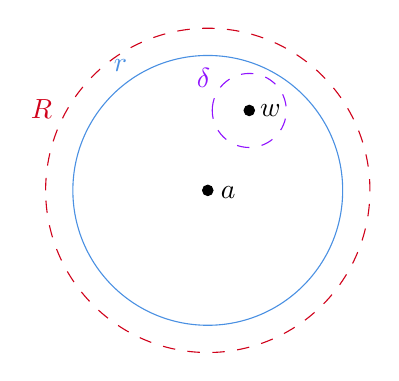
\begin{tikzpicture}[x=0.75pt,y=0.75pt,yscale=-1,xscale=1]
%uncomment if require: \path (0,300); %set diagram left start at 0, and has height of 300

%Shape: Circle [id:dp18825895148913352] 
\draw  [color={rgb, 255:red, 208; green, 2; blue, 27 }  ,draw opacity=1 ][dash pattern={on 4.5pt off 4.5pt}] (174.38,97.5) .. controls (174.38,54.35) and (209.35,19.38) .. (252.5,19.38) .. controls (295.65,19.38) and (330.63,54.35) .. (330.63,97.5) .. controls (330.63,140.65) and (295.65,175.62) .. (252.5,175.62) .. controls (209.35,175.62) and (174.38,140.65) .. (174.38,97.5) -- cycle ;
%Shape: Circle [id:dp8728584687593086] 
\draw  [fill={rgb, 255:red, 0; green, 0; blue, 0 }  ,fill opacity=1 ] (250,97.5) .. controls (250,96.12) and (251.12,95) .. (252.5,95) .. controls (253.88,95) and (255,96.12) .. (255,97.5) .. controls (255,98.88) and (253.88,100) .. (252.5,100) .. controls (251.12,100) and (250,98.88) .. (250,97.5) -- cycle ;
%Shape: Circle [id:dp10489496235227858] 
\draw  [color={rgb, 255:red, 74; green, 144; blue, 226 }  ,draw opacity=1 ] (187.5,97.5) .. controls (187.5,61.6) and (216.6,32.5) .. (252.5,32.5) .. controls (288.4,32.5) and (317.5,61.6) .. (317.5,97.5) .. controls (317.5,133.4) and (288.4,162.5) .. (252.5,162.5) .. controls (216.6,162.5) and (187.5,133.4) .. (187.5,97.5) -- cycle ;
%Shape: Circle [id:dp9134235647013942] 
\draw  [fill={rgb, 255:red, 0; green, 0; blue, 0 }  ,fill opacity=1 ] (270,59) .. controls (270,57.62) and (271.12,56.5) .. (272.5,56.5) .. controls (273.88,56.5) and (275,57.62) .. (275,59) .. controls (275,60.38) and (273.88,61.5) .. (272.5,61.5) .. controls (271.12,61.5) and (270,60.38) .. (270,59) -- cycle ;
%Shape: Circle [id:dp2734402369917359] 
\draw  [color={rgb, 255:red, 144; green, 19; blue, 254 }  ,draw opacity=1 ][dash pattern={on 4.5pt off 4.5pt}] (254.66,59) .. controls (254.66,49.15) and (262.65,41.16) .. (272.5,41.16) .. controls (282.35,41.16) and (290.34,49.15) .. (290.34,59) .. controls (290.34,68.85) and (282.35,76.84) .. (272.5,76.84) .. controls (262.65,76.84) and (254.66,68.85) .. (254.66,59) -- cycle ;

% Text Node
\draw (257.5,98.5) node [anchor=west] [inner sep=0.75pt]    {$a$};
% Text Node
\draw (166,52.4) node [anchor=north west][inner sep=0.75pt]  [color={rgb, 255:red, 208; green, 2; blue, 27 }  ,opacity=1 ]  {$R$};
% Text Node
\draw (206,33.4) node [anchor=north west][inner sep=0.75pt]  [color={rgb, 255:red, 74; green, 144; blue, 226 }  ,opacity=1 ]  {$r$};
% Text Node
\draw (276.5,59) node [anchor=west] [inner sep=0.75pt]    {$w$};
% Text Node
\draw (246,37.4) node [anchor=north west][inner sep=0.75pt]  [color={rgb, 255:red, 144; green, 19; blue, 254 }  ,opacity=1 ]  {$\delta $};


\end{tikzpicture}

\end{center}

Then if $|z - w| < \delta$, $|z - a| \leq |z - w| + |w - a| < \delta + |w - a| < r$, so $D(w, \delta) \subset D(a, r)$, and thus $\sum_{n =0}^{\infty} c_n (z - a)^n$ converges uniformly on $D(w, \delta)$.

This inspires a helpful definition.

\begin{definition}[Open]
    A subset $U$ of $\C$ is \vocab{open} if for all $w \in U$ there exists $\delta > 0$ such that $D(w, \delta) \subset U$.
\end{definition}

\begin{definition}[Local Uniform Convergence]
    Let $U$ be an open subset of $\C$ and $f_n$ be a sequence of functions on $U$. We say that $f_n$ \vocab{converges locally uniformly} on $U$ if for all $w \in U$ there exists some $\delta > 0$ such that $f_n$ converges uniformly on $D(w, \delta) \subset U$.  
\end{definition}

With this the result we discussed above can be stated as follows.

\begin{theorem}[Local Uniform Convergence of Power Series]
    A power series centered at $a$ with radius of convergence $R$ converges locally uniformly on $D(a, R)$.
\end{theorem}

We will return to this when we discuss compactness later on.

\subsection{Uniform Continuity}

Recall the standard notion of continuity.

\begin{definition}[Continuity]
	Let $A \subseteq \C$ and $f: A \rightarrow \C$. We say that $f$ is \vocab{continuous at $a$} $\in A$ if given any $\epsilon > 0$ we can find a $\delta > 0$ such that $|f(a) - f(x)| < \epsilon$ for all $x \in A$ such that $|x -a | < \delta$.


	We say that $f$ is \vocab{continuous} if it is continuous at every $a \in A$.
\end{definition}

In the above definition, our $\delta$ is allowed to depend on both $\varepsilon$ \emph{and} $x$.

\begin{definition}[Uniform Continuity]
    Let $A \subset \C$ and $f: A \rightarrow \C$. We say that $f$ is \vocab{uniformly continuous} on $A$ if given any $\varepsilon > 0$ we can find a $\delta > 0$ such that for all $x, y \in U$ we have $|x - y| < \delta$ implying $|f(x) - f(y)| < \varepsilon$.
\end{definition}

Here, we again impose this \emph{uniformity} constraint, that is, $\delta$ is allowed to depend on $\varepsilon$ only. 

It's easy to see that uniform continuity implies continuity, but the converse doesn't hold in general.

\begin{example}[Uniformly Continuous Function]
    We will show that $f(x) = 2x + 17$ is uniformly continuous over $\R$. 

    Given $\varepsilon > 0$, let $\delta = \varepsilon / 2$. Then for all $x, y \in \R$ with $|x - y| < \delta$ we have $|f(x) - f(y)| = 2|x - y| < \varepsilon$, as required.
\end{example}

\begin{example}[A Non-Uniformly Continuous Function]
    The function $f(x) = x^2$ over $\R$ is continuous, but not uniformly continuous. 

    Consider $\varepsilon = 1$. Then given some $\delta$, let $x > 1/\delta$ and $y = 1/\delta + \delta/2$. Then we have $|x - y| < \delta$ but $|f(x) - f(y)| = 1 + \delta^2/4 > 1 = \varepsilon$, so $f$ is not uniformly continuous.
\end{example}

Here, our uniform continuity was shown to not hold by taking larger and larger $x$, which forced the slope of the function to get too large for a given value of $\delta$ to be sufficient. It turns out that this is the only failure point of uniform continuity, and indeed continuity implies uniform continuity when we are working over a bounded interval.

The proof of this is quite natural -- we use Bolzano-Weierstrass to show that a contradiction to uniform continuity is a contradiction to continuity.\footnote{Another argument which is more direct can be made using compactness, but we will look past this for now.}

\begin{theorem}[Continuous Functions are Uniformly Continuous]
    Let $f: [a, b] \rightarrow \C$ be continuous. Then $f$ is uniformly continuous
\end{theorem}
\begin{proof}
	Suppose $f$ was not uniformly continuous, that is, there exists some $\epsilon > 0$ such that for all $\delta > 0$ there is some $x, y$ with $|x - y| < \delta$ such that $|f(x) - f(y)| \geq \epsilon$.

	Taking $\delta = 1/n$, we can find some sequences $x_n, y_n \in [a, b]$ such that $|x_n - y_n| < 1/n$, and $|f(x_n) - f(y_n)| \geq \epsilon$. Then by Bolzano-Weierstrass, we can find some convergent subsequence $x_{n_j} \rightarrow x$ for some $x \in [a, b]$. But then $|x_{n_j} - y_{n_j}| < 1/n_j$ for all $j$, so we must have $y_{n_j} \rightarrow x$ also.

	Then $|f(x_{n_j}) - f(y_{n_j})| \geq \epsilon$ for every $j$, which implies that $f(x_{n_j})$ and $f(y_{n_j})$ cannot converge to the same value. But then by continuity we have $f(x_{n_j}) \rightarrow f(x)$ and $f(y_{n_j}) \rightarrow f(x)$, which is a contradiction. Thus $f$ must be uniformly continuous.
\end{proof}

With this result, we can prove the familiar result that continuous functions are integrable.

\begin{theorem}[Continuous Functions are Integrable]
	Let $f:[a, b] \rightarrow \R$ be continuous. Then $f$ is Riemann integrable.
\end{theorem}
\begin{proof}
	Given $\epsilon > 0$, since $f$ is uniformly continuous, there is some $\delta > 0$ such that $|f(x) - f(y)| < \epsilon/(b - a)$ whenever $|x - y| < \delta$ and $x, y \in [a, b]$.

	Now choose some integer $n \geq (b - a)/\epsilon$, and define the dissection $\DD = \{x_0, x_1, \dots, x_n\}$ with $x_j = a + j(b - a)/n$. Then we have
	$$
	\sup_{x \in [x_{j - 1}, x_j]} f(x) - \inf_{x \in [x_{j - 1}, x_j]} f(x) \leq \frac{\epsilon}{(b - a)},
	$$
	for all $1 \leq j \leq n$, and thus 
	\begin{align*}
		S_\DD(f) - s_\DD(f) &= \sum_{j = 1}^n (x_j - x_{j - 1})\left[\sup_{x \in [x_{j - 1}, x_j]} f(x) - \inf_{x \in [x_{j - 1}, x_j]} f(x)\right] \\
		&\leq \sum_{j = 1}^n \frac{b - a}{n} \cdot \frac{\epsilon}{b - a} = \epsilon,
	\end{align*}
	and thus $f$ is Riemann integrable.
\end{proof}

\section{Metric Spaces}

\subsection{Defining Metric Spaces}

In $\R$ and $\C$, we measured the `closeness' of two points $x, y$ using $|x - y|$. We used this throughout our study of analysis both in this course and previously, and possibly the most important property of this was the triangle inequality,
$$
|x + z| \leq |x + y| + |y + z|.
$$

The triangle inequality acts, more or less, as saying that being close is \emph{transitive}. That is, if $x$ is close to $y$, and $y$ is close to $z$, then $x$ is close to $z$.

In fact, we can abstract away quite naturally from the absolute value into a more general setting in which a measure of distance has this property.

\begin{definition}[Metric]
    Let $M$ be a set. A \vocab{metric} on $M$ is a function $d: M \times M \rightarrow \R$ such that
    \begin{itemize}
        \item \emph{Positivity}. For all $x, y \in M$, $d(x, y) \geq 0$, with equality if and only if $x = y$.
        \item \emph{Symmetry}. For all $x, y \in M$, $d(x, y) = d(y, x)$.
        \item \emph{Triangle inequality}. For all $x, y, z \in M$,
        $$
        d(x, z) \leq d(x, y) + d(y, z).
        $$
    \end{itemize}
\end{definition}

\begin{definition}[Metric Space]
    A \vocab{metric space} is a pair $(M, d)$ where $M$ is a set and $d$ is a metric on $M$. 
\end{definition}

\begin{example}[Metric Spaces on $\R$]
    The real line $\R$ is a metric space under the metric $d(x, y) = |x - y|$. In fact, any subset of $\R$ is a metric space with the same metric.
\end{example}

\begin{example}[Euclidean Space $\R^n$]
   In $\R^n$, we can define the \vocab{Euclidean norm}
   of $x \in \R^n$ by
   $$
    \norm{x} = \norm{x}_2 = \left(\sum_{k = 1}^n |x_k|^2\right)^{\frac{1}{2}}.
   $$
   This satisfies the triangle inequality $\norm{x + y} \leq \norm{x} + \norm{y}$. This `norm' then induces a metric on $\R^n$
   $$
    d(x, y) = d_2(x, y) = \norm{x - y}_2 = \left(\sum_{k = 1}^n |x_k - y_k|^2\right)^{\frac{1}{2}}.
   $$
   This metric is the \vocab{Euclidean distance}, and with it we get a metric space $(\R^n, d_2)$ called \vocab{Euclidean space}. This is the standard metric space on $\R^n$.
\end{example}
\begin{remark}
    We sometimes denote the $n$-dimensional real or complex Euclidean space by $\ell_2^n$. The Euclidean norm is called the $\ell_2$-norm, and the corresponding Euclidean distance is called the $\ell_2$-metric.
\end{remark}

\begin{example}[Taxicab Metric]
It's also possible to use the \vocab{taxicab metric} on $\R^n$, given by
$$
d(x, y) = \sum_{k = 1}^{n} |x_k - y_k|.
$$
This is also known as the $\ell_1$-metric.
\end{example}

\begin{example}[$\ell_\infty$ Metric]
In $\R^n$ or $\C^n$, we can define the $\ell_{\infty}$ norm of $x$ by
$$
    \norm{x}_{\infty} = \max_{1 \leq k \leq n} |x_k|,
$$
and then we can define the \vocab{$\ell_{\infty}$-metric} by
$$
d(x, y) = \norm{x - y}_{\infty} = \max_{1 \leq k \leq n} |x_k - y_k|.
$$
We then get a metric space which we denote by $\ell_{\infty}^n$.
\end{example}

\begin{example}[Uniform Metric]
    Let $S$ be a set, and let $\ell_{\infty}(S)$ be the set of all bounded scalar functions on $S$. We define the $\ell_{\infty}$-norm of $f \in \ell_{\infty}(S)$ by
    $$
    \norm{f} = \norm{f}_{\infty} = \sup_{x \in S}|f(x)|,
    $$
    also called the $\sup$ norm or the uniform norm. From this we can define $d(f, g) = \norm{f - g}_{\infty}$ called the \vocab{uniform metric} on $\ell_{\infty}(S)$.
\end{example}

\begin{example}[$L_p$-Norm]
    Let $\mathcal{C}[a, b]$ be the set of all continuous functions defined on the closed and bounded interval $[a, b]$. Then for $p \geq 1$ we can define the \vocab{$L_p$-norm} of $f \in \mathcal{C}[a, b]$ by
    $$
    \norm{f}_p = \left(\int_a^b |f(x)|^p \dd x\right)^{1/p}.
    $$
    This defines\footnote{If you want to check that $d_p$ satisfies the metric space axioms, you do need the \emph{Minkowski inequality}, which we will not discuss.} the \vocab{$L_p$-metric}, $d_p(f, g) = \norm{f - g}_{p}$.
\end{example}

\begin{example}[Discrete Metric]
Let $M$ be any set. Then
$$
d(x, y) = \begin{cases}
    0 &\mbox{if } x = y, \\
    1 &\mbox{if } x \neq y.
   \end{cases}
$$
defines the metric called the \vocab{discrete metric}, and $(M, d)$ is called a \vocab{discrete metric space}.
\end{example}

\begin{example}[Word Metric]
    Let $G$ be a group generated by $S \subset G$, where $e \not \in S$ and $x \in S$ implies $x^{-1} \in S$. Then
    $$
    d(x, y) = \min \{n \geq 0 \mid \text{there exists } s_1, \dots, s_n \in S \text{ such that } y = x s_1 \cdots s_n \}
    $$
    defines the \vocab{word metric}.
\end{example}

\begin{example}[$p$-adic Metric]
    Fix a prime $p \in \N$. We define
    $$
    d(x, y) = \begin{cases}
        0 &\mbox{if } x = y, \\
        p^{-n} &\mbox{if } x \neq y \text{ where }x - y = p^n m.
       \end{cases}
    $$
    defines a metric on $\Z$ called the \vocab{$p$-adic metric}.
\end{example}

\subsection{Subspaces}

As with many mathematical objects, it can be useful to discuss the substructure to a metric space.

\begin{definition}[Subspace]
    Let $(M, d)$ be a metric space and let $N \subset M$. Then $d$ is a metric on $N$, and $(N, d)$ is a \vocab{subspace} of $M$.    
\end{definition}

\begin{example}[$\Q$ is a subspace of $\R$]
$\Q$ with the metric $d(x, y) = |x - y|$ is a subspace of $\R$.   
\end{example}

\begin{example}[$\mathcal{C}{[a, b]}$ is a subspace of $\ell_{\infty}({[a, b]})$]
    Since every continuous function on a closed, bounded interval is bounded, it follows that $\mathcal{C}[a, b]$ is a subset of $\ell_{\infty}([a, b])$, so $\mathcal{C}[a, b]$ with the uniform metric is a subspace of $\ell_{\infty}([a, b])$.
\end{example}

Given two metric spaces, there is a number of natural construction of another metric space which has those two metric spaces as subspaces.

\begin{definition}[Product Space]    
    Let $(M, d)$ and $(M', d')$ be metric spaces. Then each of the following defines a metric on $M \times M'$:
    \begin{align*}
        d_1((x, x'), (y, y')) &= d(x, y) + d'(x', y') ,\\
        d_2((x, x'), (y, y')) &= \left(d(x, y)^2 + d'(x', y')^2\right)^{1/2} ,\\
        d_{\infty}((x, x'), (y, y')) &= \max\{d(x, y), d'(x', y')\}.
    \end{align*}
    We denote the metric space $(M \times M', d_p)$ by $M \oplus_p M'$.
\end{definition}

\begin{remark}
    There is no canconical choice of which of $\{d_1, d_2, d_{\infty}\}$ we take as the product metric. Indeed, it's straightforward to show that
    $$
    d_{\infty} \leq d_2 \leq d_1 \leq 2 d_{\infty},
    $$
    and later on when we discuss concepts such as convergence we will see that because of this fact, the exact choice of metric doesn't matter \emph{that} much.
\end{remark}

Of course, this construction extends naturally to any finite number of metric spaces.

\subsection{Convergence}

Metric spaces give us a measure of closeness, and we know that in $\R$ and $\C$ that convergence is really just a notion of a sequence getting close to some `limiting value'. Indeed, convergence as we defined it before directly translates into the language of metric spaces.

\begin{definition}[Convergence]
    Let $(M, d)$ be a metric space. A sequence $a_1, a_2, \dots \in M$ is said to \vocab{converge} to the limit $a \in M$ if given any $\varepsilon > 0$, we can find an integer $N$ such that $d(a_n, a) < \varepsilon$ for all $n \geq M$. We write $a_n \rightarrow a$ as $n \rightarrow \infty$.
\end{definition}

A straightforward but useful thing to note is that this definition implies $a_n \rightarrow a$ if and only if $d(a_n, a) \rightarrow 0$ in $\R$.

Now we need to go back to all of the theorems about convergence that were proved in an earlier Analysis course and check if they still hold for a general Metric space (that is, if they don't really use the structure of $\R$, apart from closeness).

\begin{lemma}[Uniqueness of Limits]
    If $a_n \rightarrow a$ and $a_n \rightarrow b$ in a metric space $M$, then $a = b$.
\end{lemma}
\begin{proof}
	Assume that $a \neq b$. Given any $\epsilon > 0$, we can find integers $N_1$ and $N_2$ such that
	\begin{align*}
		d(a_n, a) \leq \epsilon, \quad \text{ for all $n \geq N_1$}\\
		d(a_n, b) \leq \epsilon, \quad \text{ for all $n \geq N_2$}
	\end{align*}
	Then letting $\epsilon = d(a, b)/3$ and taking $N = \max\{N_1, N_2\}$, we have by the triangle inequality
	$$
	d(a, b) \leq d(a, a_n) + d(a_n, b) \leq 2\epsilon = \frac{2}{3} d(a, b)
	$$
	for all $n \geq N$.
	Thus we must have $d(a, b) = 0$, and $a = b$, contradicting our assumption.
\end{proof}

\begin{lemma}[Convergence of Subsequences]
    If $a_n \rightarrow a$ as $n \rightarrow \infty$ in a metric space $M$, and $n(1) < n(2) < \cdots$, then $a_{n(j)} \rightarrow a$ as $j \rightarrow \infty$.
\end{lemma}
\begin{proof}[Proof Sketch]
    Take the old proof from $\R$ and $\C$ and replace the absolute values with the metric!
\end{proof}

\subsection{Continuity}

As with convergence, we also get a direct generalization of the notion of continuity.

\begin{definition}[Continuity]
    Let $f: M \rightarrow M'$ be a function between metric spaces $(M, d)$ and $(M', d')$. Then for $a \in M$, we say that $f$ is \vocab{continuous} at $a$ if given any $\varepsilon > 0$ we can find a $\delta > 0$ such that $d'(f(x), f(a)) < \varepsilon$ for all $x \in M$ such that $d(x, a) < \delta$.

    We say that $f$ is \vocab{continuous} if $f$ is continuous at $a$ for all $a \in M$.
\end{definition}

\begin{proposition}[Sequence Definition of Continuity]
    Let $f: M \rightarrow M'$ be a function between metric spaces, and let $a \in M$. 
    Then $f$ is continuous at $a$ if and only if $x_n \rightarrow a$ in $M$ implies that $f(x_n) \rightarrow f(a)$ in $M'$.
\end{proposition}

We also keep the same standard properties of continuity as before.

\begin{proposition}[Sums, Products, and Reciporicals of Continuous Functions]
	Let $f, g: M \rightarrow M'$ be scalar functions on metric spaces $M$ and $M'$. Then the following hold.
	\begin{enumerate}[label=(\roman*)]
		\item If $f$ and $g$ are continuous at $a$, then so is their sum $f + g$.
		\item If $f$ and $g$ are continuous at $a$, then so is their product $fg$.
		\item If $N = \{x \in M \mid g(x)\neq 0\}$, then if $f$ and $g$ are continuous at $a \in N$, then so is $f/g$.
	\end{enumerate}
\end{proposition}

\begin{proposition}[The Composition of Continuous Functions is Continuous]
	Let $f: M \rightarrow M'$ and $g: M' \rightarrow M''$ with $M, M', M''$ all metric spaces. Then if $f$ is continuous at $a \in M$ and $g$ is continuous at $f(a)$, then $g \circ f$ is also continuous at $a$.
\end{proposition}

\begin{example}[Constant Function]
    Consider the constant function $f: M \rightarrow M'$ with $f(x) = b$ for some $b \in M'$. Then $f$ is continuous.
\end{example}

\begin{example}[Identity Function]
    Consider the identity function $\operatorname{id}: M \rightarrow M$. This is continuous at all $a \in M$, as given $\varepsilon > 0$ we can take $\delta = \varepsilon$, and if $d(x, a) < \delta$ then $d(\operatorname{id}(x), \operatorname{id}(a)) = d(x, a) < \delta = \varepsilon$.
\end{example}

\begin{example}[Polynomials]
    Using the examples above, we get that polynomials are always continuous.
\end{example}

\begin{example}[Metrics are Continuous]
    Let $(M, d)$ be a metric space. Then $d$ is a function between metric spaces, $d: M \oplus_p M \rightarrow \R$ (where we take some $p \in \{1, 2, \infty\}$).

    Given $v = (x, x')$ and $w = (w, w') \in M \oplus_p M$, then 
    $$|d(v) - d(w)| = |d(x, x') - d(y, y')| \leq d(x, y) + d(x', y') = d_1(v, w) \leq 2d_p(v, w)$$
    So $\delta = \varepsilon/2$ will do.
\end{example}

\begin{definition}[Isometric and Lipschitz]
    Let $f: M \rightarrow M'$ be a function between metric spaces. Then $f$ is \vocab{isometric} if for all $x, y \in M$ we have $d'(f(x), f(y)) = d(x, y)$.

    We say that $f$ is \vocab{Lipschitz} if there exists some $c \in \R^+$ such that $d'(f(x), f(y)) \leq cd(x, y)$.
\end{definition}

\begin{definition}[Uniform Continuity]
    Let $f: M \rightarrow M'$ be a function between metric spaces. We say that $f$ is \vocab{uniformly continuous} if given $\varepsilon > 0$, there exists some $\delta > 0$ such that for all $x, y \in M$ with $d(x, y) < \delta$ we have $d'(f(x), f(y)) < \varepsilon$. 
\end{definition}

We can easily see that $f$ isometric implies that it's Lipschitz, and $f$ Lipschitz implies that it's uniformly continuous. Also, if $f$ is isometric then it must be injective (but not necessarily surjective). If $f$ is also surjective then we call it a \vocab{isometry}.

If there exists an isometry between two metric spaces $M$ and $M'$, we say that they are \vocab{isometric}.

\begin{example}
    Let $(M,d)$ and $(M', d')$ be metric spaces, and fix some $y \in M'$. Then if we define $f: M \rightarrow M \oplus_p M'$ by $f(x) = (x, y)$, we have $d_p(f(x), f(z)) = d_p((x, y), (x, z)) = d(x, z)$. So $f$ is an isometry, and $M \times \{y\}$ is an isometric copy of $M$ in the space $M \oplus_p M'$. 
\end{example}

\subsection{The Topology of a Metric Spaces}

While we will discuss topology and topological spaces later, it's worth looking at a few of the core ideas in the context of metric spaces.

It seems that there are some concepts in metric spaces that don't \emph{really} rely on the metric, just about the closeness of points. The point of this section is looking to see exactly what type of relations are these, so that we can generalize them to a setting where we don't use a metric.

We begin with the familiar concept of an open ball.

\begin{definition}[Open Ball]
    Let $M$ be a metric space, $x \in M$ and $r > 0$. The \vocab{open ball} in $M$ of center $x$ and radius $r$ is the set $D_r(x)$ given by
    $$
    D_r(x) = \{y \in M \mid d(x, y) < r \}.
    $$
\end{definition}

The idea of open balls is a natural one, and it even fits naturally into some of our previous definitions.

For example, we say that $x_n \rightarrow x$ in $M$ if and only if for all $\varepsilon > 0$, there is some positive integer $N$ such that $n \geq N$ implies that $x_n \in D_{\varepsilon}(x)$.

Similarly, for a function $f: M \rightarrow M'$ we say that $f$ is continuous at $x \in M$ if and only if for all $\varepsilon > 0$ there exists some $\delta > 0$ such that $f(D_{\delta}(x)) \subset D_{\varepsilon}(f(x))$.

\begin{definition}[Closed Ball]
    Let $M$ be a metric space, $x \in M$ and $r > 0$. The \vocab{closed ball} in $M$ of center $x$ and radius $r$ is the set $B_r(x)$ given by
    $$
B_r(x) = \{y \in M \mid d(x, y) \leq r\}.
    $$
\end{definition}

\begin{example}[Open and Closed Ball in $\R$]
    In $\R$, we have $D_r(x) = (x - r, x + r)$, and $B_r(x) = [x - r, x + r]$.
\end{example}

We now move to define some concepts that will be a little less straightforward, but should come together later on as we discuss more topology.

\begin{definition}[Neighborhood]
    Let $M$ be a metric space, and let $U \subset M$. For $x \in M$, we say that $U$ is a \vocab{neighborhood} of $x$ in $M$ if there exists some $r > 0$ such that $D_r(x) \subset M$.
\end{definition}
\begin{definition}[Open]
    We say that $U$ is \vocab{open} in $M$ if for all $x$ in $U$ there is some $r > 0$ such that $D_r(x) \subset U$. That is, if $U$ is a neighborhood for all of its points.
\end{definition}

\begin{example}[Upper Half of the Complex Plane is Not Open]
    Consider the set $H = \{z \in C \mid \im z \geq 0 \}$.
    Then let $w \in H$, and let $\delta = \im w$. If $\delta > 0$, then $D_{\delta}(w) \subset H$, and if $\delta = 0$, then for all $r > 0$ $D_r(w) \not \subset H$. Thus $H$ is not open.
\end{example}

We commonly use the seeming tautological fact that open balls are open.

\begin{lemma}
    Open balls are open.
\end{lemma}
\begin{proof}
    Consider some open ball $D_r(x)$ in a metric space $M$. Then let $y \in D_r(x)$, and set $\delta = r - d(x, y)$. Then $\delta >0$, and if $z \in D_{\delta}(y)$ then
    $$
    d(z, x) \leq d(z, y) + d(y, x) < \delta + d(x, y) = r,
    $$
    so $z \in D_r(x)$. This shows that $D_{\delta}(y) \subset D_r(x)$.
\end{proof}

\begin{corollary}
    Let $M$ be a metric space, $U \in M$ and $x \in M$. Then $U$ is a neighborhood of $x$ if and only if there exists an open subset $V$ of $M$ such that $x \in V \subset U$.
\end{corollary}
\begin{proof}[Proof Sketch]
    Check definitions.
\end{proof}

This notion of neighborhoods and open sets is sufficient to describe both convergence and continuity in a metric space on its own.

\begin{proposition}[Convergence using Open Sets \& Neighborhoods]
    In a metric space $M$, the following are equivalent.
    \begin{enumerate}[label=(\roman*)]
        \item $x_n \rightarrow x$;
        \item For all neighborhoods $U$ of $x$ in $M$, there exists some positive integer $N$ such that $n \geq N$ implies $x_n \in U$;
        \item For all open subsets $U$ of $M$ with $x \in U$, there is a positive integer $N$ such that for all $n \geq N$ we have $x_n \in U$.
    \end{enumerate}
\end{proposition}
\begin{proof}
    \emph{(i) implies (ii)}. Let $U$ be a neighborhood of $x$ in $M$. Then by definition there exists some $\varepsilon > 0$ such that $D_{\varepsilon}(x) \subset U$. Then since $x_n \rightarrow x$, there's an $N \in \N$ such that $n \geq N$ implies $d(x_n, n) < \varepsilon$, that is, $x_n \in D_{\varepsilon}(x)$. 

    \emph{(ii) implies (iii)}. This is clear since any open set $U$ with $x \in U$ is a neighborhood of $x$.

    \emph{(iii) implies (i)}. Given some $\varepsilon > 0$, $U = D_{\varepsilon}(x)$ is open and $x \in U$. Then by (iii) there's an $N \in \N$ such that $n \geq N$ implies $x_n \in U$, that is, $d(x_n, x) < \varepsilon$.
\end{proof}

\begin{proposition}[Local Continuity using Open Sets \& Neighborhoods]
    Let $f: M \rightarrow M'$ be a function between metric spaces, and let $x \in M$. Then the following are equivalent:
    \begin{enumerate}[label=(\roman*)]
        \item $f$ is continuous at $x$;
        \item For all neighborhoods $V$ of $f(x)$ in $M'$, there exists a neighborhood $U$ of $x$ in $M$ such that $f(U) \subset V$;
        \item For all neighborhoods $V$ of $f(x)$ in $M'$, $f^{-1}(V)$ is a neighborhood of $x$ in $M$.
    \end{enumerate}
\end{proposition}
\begin{proof}
    \emph{(i) implies (ii)}. Let $V$ be a neighborhood of $f(x)$ in $M'$. Then by definition there exists some $\varepsilon > 0$ such that $D_{\varepsilon}(f(x)) \subset V$. Since $f$ is continuous at $x$, there exists $\delta > 0$ such that $f(D_{\delta}(x)) \subset D_\varepsilon(f(x))$. Then $U = D_{\delta}(x)$ is a neighborhood of $x$ in $M$, and $f(U) \subset V$.

    \emph{(ii) implies (iii)}. Let $V$ be a neighborhood of $f(x)$ in $M'$. Then by (ii) there is a neighborhood $U$ of $x$ in $M$ such that $f(U) \subset V$. Then $U \subset f^{-1}(V)$, and since $U$ is a neighborhood of $x$ in $M$, there is some $r > 0$ with $D_r(x) \subset U \subset f^{-1}(V)$. Thus $f^{-1}(V)$ is a neighborhood of $x$ in $M$.

    \emph{(iii) implies (i)}.
    Given $\varepsilon > 0$, $V = D_{\varepsilon}(f(x))$ is a neighborhood of $f(x)$ in $V$. By (iii), $f^{-1}(V)$ is a neighborhood of $x$ in $M$. So there exits $\delta > 0$ with $D_{\delta}(x) \subset f^{-1}(V)$. Then $f(D_{\delta}(x)) \subset V = D_{\delta}(f(x))$.
\end{proof}

\begin{proposition}[Global Continuity using Open Sets \& Neighborhoods]
    Let $f: M \rightarrow M'$ be a function between metric spaces. Then the following are equivalent:
    \begin{enumerate}[label=(\roman*)]
        \item $f$ is continuous;
        \item $f^{-1}(V)$ is open in $M$ for all open subsets $V$ of $M'$.
    \end{enumerate}
\end{proposition}
\begin{proof}
    \emph{(i) implies (ii)}. Let $V$ be open in $M'$. Let $x \in f^{-1}(V)$. Then $f(x) \in V$. Since $V$ is open, there's some $\varepsilon > 0$ such that $D_{\varepsilon}(f(x)) \subset V$. Since $f$ is continuous at $x$, there's a $\delta > 0$ such that $f(D_{\delta}(x)) \subset D_{\varepsilon}(f(x))$. Therefore $D_{\delta}(x) \subset f^{-1}(D_\varepsilon (f(x))) \subset f^{-1}(V)$. Thus $f^{-1}(V)$ is open in $M$.

    \emph{(ii) implies (i)}. Let $x \in M$, and let $\varepsilon > 0$. Then $V = D_{\varepsilon}(f(x))$ is open in $M'$. By (ii) $f^{-1}(V)$ is open in $M$, also $x \in f^{-1}(V)$ and $f(x) \in V$. Then by definition there's a $\delta > 0$ such that $D_{\delta}(x) \subset f^{-1}(V)$, so $f(D_{\delta}(x)) \subset V = D_\varepsilon(f(x))$.
\end{proof}

We can now write down what the \emph{topology} of a metric space is. We are going to study topology in general later on, but we can use some properties that occur here to inform how we define things more generally afterwards.

\begin{definition}[Topology of a Metric Space]
    The \vocab{topology} of a metric space $M$ is the family of all open subsets of $M$.
\end{definition}

\begin{proposition}[Basic Properties]
    The topology of a metric space satisfies the following.
    \begin{enumerate}[label=(\roman*)]
        \item $\emptyset$ and $M$ are open.
        \item If $U_i$ is open in $M$ for all $i$ in some index set $I$, then $\bigcup_{i \in I} U_i$ is open in $M$.
        \item $U, V$ open in $M$ implies $U \cap V$ open in $M$.
    \end{enumerate}
\end{proposition}
\begin{proof}
    \emph{Part (i)}. This is clear.

    \emph{Part (ii)}. Given $x \in \bigcup_{i \in I} U_i$, then there's some $i_0 \in I$ with $x \in U_{i_0}$. Then $U_{i_0}$ is open, so by definition there's an $r > 0$ with $D_r(x) \subset U_{i_0} \subset \bigcup_{i \in I} U_i$.

    \emph{Part (iii)}. Given $x \in U \cap V$, since $U$ is open and $x \in U$, there's an $r > 0$ with $D_r(x) \subset U$, and since $V$ is open and $x \in V$, there's an $s > 0$ with $D_s(x) \subset V$. Then letting $t = \min\{r, s\}$, we have $t >0$ and $D_t(x) = D_r(x) \cap D_s(x) \subset U \cap V$.
\end{proof}

\begin{definition}[Closed]
    A subset $A$ of a metric space $M$ is \vocab{closed} in $M$ if for every sequence $x_n \in A$ that is convergent in $M$, we have $\lim_{n \to \infty} x_n \in A$.
\end{definition}

\begin{lemma}
    Closed balls are closed.
\end{lemma}
\begin{proof}
    Consider $B_r(x) = \{y \in M \mid d(y, x) \leq r\}$ in a metric space $M$, and a sequence $x_n \in B_r(x)$ such that $x_n \rightarrow z$. We need to show that $z \in B_r(x)$. We have
    \begin{align*}
        d(z, x) &\leq d(z, x_n) + d(x_n, x) \\
            &\leq d(z, x_n) + r \rightarrow r
    \end{align*}
    as $n \rightarrow \infty$. Thus $d(z, x) \leq r$, and hence $z \in B_r(x)$.
\end{proof}

\begin{example}[Closed but Not Open, and Open but Not Closed Sets]
    The set $[0, 1] = B_{\frac{1}{2}}(1/2)$ is closed in $\R$. $[0, 1]$ is not open, for example $D_r(0) \not \subset [0, 1]$ for any $r > 0$.

    The set $(0, 1) = D_{\frac{1}{2}}(1/2)$ is open, but it is not closed. Take $1/(n + 1) \in (0, 1)$ for all $n \in \N$. Then $1/(n + 1) \rightarrow 0$ in $\R$ but $0 \not \in (0, 11)$.
\end{example}

\begin{example}[An Open and Closed Set]
   $\R$ is open and closed in $\R$.
\end{example}

\begin{example}[A Neither Open or Closed Set]
    The set $(0, 1]$ in $\R$ is neither open nor closed.
\end{example}

\begin{lemma}[Relating Closed and Open]
    Let $A$ be a subset of a metric space $M$. Then $A$ is closed in $M$ if and only if $M \backslash A$ is open in $M$.
\end{lemma}
\begin{proof}
    Assume $A$ is closed, and that $M \backslash A$ is not open. Then there exists $x \in M \backslash A$ such that for all $r > 0$ we have $D_r(x) \not \subset M\backslash A$. 
    Hence for all $n$ there exists $x_n \in D_{1/n}(x) \cap A$. Then $d(x_n, x) < 1/n \rightarrow 0$, so $x_n \rightarrow x$ in $M$ and $x_n \in A$ for all $n$, which contradicts that $A$ is closed.

    Now suppose that $M \backslash A$ is open but $A$ is not closed. Then there exists some sequence $x_n$ in $A$ such that $x_n \rightarrow x$ in $M$ but $x \not \in A$. Since $x \in M \backslash A$ and $M \backslash A$ is open, there exists $\varepsilon > 0$ with $D_\varepsilon(x) \subset M \backslash A$. Then since $x_n \rightarrow x$, there is some $N \in \N$ such that for all $n \geq N$ we have $x_ \in D_{\varepsilon}(x)$, and hence $x_n \in M \backslash A$, which is a contradiction.
\end{proof}

We previously met isometries, which were maps between metric spaces that preserved the distance function. Now that we are trying to look slightly away from metrics and more towards open sets and neighborhoods, it's natural to think of a new definition of a function between metric spaces that preserves open sets.

\begin{definition}[Homeomorphism]
    A map $f: M \rightarrow M'$ between metric spaces is a \vocab{homeomorphism} if $f$ is a bijection, and $f$ and $f^{-1}$ are both continuous.

    Equivalently, $f$ is a homeomorphism if for all open sets $V$ in $M'$, $f^{-1}(V)$ is open in $M$, and for all open sets $U$ in $M$, $f(U)$ is open in $M'$.

    If there is a homeomorphism between $M$ and $M'$, we say that $M$ and $M'$ are \vocab{homeomorphic}.
\end{definition}

\begin{example}
    The metric spaces $(0, \infty)$ and $(0, 1)$ are homeomorphism with the homeomorphism $x \mapsto 1/(x + 1)$ and inverse $x \mapsto 1/x - 1$.
\end{example}

While is is true that every isometry is a homeomorphism, the converse is absolutely false.

We will say that two metrics on a set are equivalent if they induce the same topology.

\begin{definition}[Equivalent Metrics]
    Let $d$ and $d'$ be metrics on a set $M$. We say that $d$ and $d'$ are \vocab{equivalent}, denoted $d \sim d'$, if they define the same topology on $M$. That is, for $U \subset M$, $U$ is open in $(M, d)$ if and only if $U$ is open in $(M, d')$.
\end{definition}

So $d \sim d'$ if and only if $\operatorname{id}: (M, d) \rightarrow (M, d')$ is a homeomorphism. 

Note that if $d \sim d'$, then $(M, d)$ and $(M, d')$ have the same convergent sequences and the same continuous maps.

\begin{definition}[Uniformly and Lipschitz Equivalent]
    Let $d$ and $d'$ be metrics on a set $M$. We say that $d$ and $d'$ are \vocab{uniformly equivalent} if $\operatorname{id}: (M, d) \rightarrow (M, d')$ and $\operatorname{id}: (M, d') \rightarrow (M, d)$ are uniformly continuous, and write $d \sim_u d'$.

    We will say $d$ and $d'$ are \vocab{Lipschitz equivalent} if these functions are Lipschitz, and write $d \sim_{Lip} d'$.
\end{definition}

Note that $d \sim_{Lip} d'$ if and only if there exists $a > 0$ and $b > 0$ such that
$$
a d(x, y) \leq d'(x, y) \leq b d(x, y),
$$
and also note that $d \sim_{Lip} d'$ implies $d \sim_u d'$ implies $d \sim d'$.

\begin{example}
    Given a metric space $(M, d)$, $d'(x, y) = \min\{1, d(x, y)\}$ defines a metric on $M$, and $d' \sim_u d$.
\end{example}

\begin{example}
    On a product space $M \times M'$, the metrics $d_1$, $d_2$ and $d_{\infty}$ are pairwise Lipschitz equivalent.
\end{example}

\begin{example}
    On $C[0, 1]$, the $L_1$-metric and the uniform metric are \emph{not} equivalent.
\end{example}

We will return to these topological ideas later on.

\section{Completeness and the Contraction Mapping Theorem}

\subsection{Completeness}

In $\R$ and $\C$ that every Cauchy sequence is convergent. In what spaces is this true?

\begin{definition}[Cauchy Sequence]
    A sequence $x_n$ in a metric space $M$ is \vocab{Cauchy} if given $\varepsilon > 0$, there's some positive integer $N$ such that $n, m \geq N$ implies that $d(x_n, x_m) < \varepsilon$.
\end{definition}

\begin{definition}[Bounded]
    A sequence $x_n$ in a metric space $M$ is \vocab{bounded} if there exists some $z \in M$ and $r > 0$ such that for all $n$ w have $x_n \in B_r(z)$.
\end{definition}

\begin{lemma}[Convergent Implies Cauchy Implies Bounded]
    Every convergent sequence is Cauchy, and every Cauchy sequence is bounded.
\end{lemma}
\begin{proof}
    Let $x_n$ be a sequence in metric space $M$. 
    
    Suppose $x_n$ is convergent in $M$, and let $x = \lim_{n \to \infty} x_n$.
    Given $\varepsilon > 0$, there is some positive integer $N$ such that $n \geq N$ implies $d(x_n, x) < \varepsilon/2$.
    Then for all $m, n \geq N$, $d(x_m, x_n) \leq d(x_m, x) + d(x, x_n) < \varepsilon$. Thus if a sequence converges, then it's Cauchy.

    Now assume that $x_n$ is Cauchy in $M$. Then there's a positive integer $N$ such that for all $m, n \geq N$ we have $d(x_m, x_n) < 1$. In particular, $d(x_n, X_N) < 1$ for $n \geq N$, that is, $x_n \in B_1(x_N)$ for $n \geq N$.
    So let $r = \max\{d(x_1, x_N), \dots, d(x_{N - 1}, x_N)\}$. Then $x_n \in B_r(x_N)$ for all $n \in \N$, and so $x_n$ is bounded.
\end{proof}

In general, being bounded does not imply that a sequence is Cauchy (for example, take the sequence $0, 1, 0, 1, \dots$).

Slightly more subtle is that being Cauchy doesn't imply convergence, and we can construct a somewhat silly example. For example, $x_n = 1/n$ is Cauchy but doesn't converge in the metric space $(0, \infty)$.
It seems that this example works because there's something `missing' from the metric space -- the limit of a sequence. Indeed, in this section we will care about metric spaces where such an implication \emph{does hold}, in `complete' metric spaces.

\begin{definition}[Completeness]
    A metric space $M$ is \vocab{complete} if every Cauchy sequence in $M$ converges in $M$.
\end{definition}

\begin{example}
    $\R$ and $\C$ are complete.
\end{example}

\begin{proposition}
    If $M$ and $M'$ are complete metric spaces, then so is $M \oplus_p M'$.
\end{proposition}
\begin{proof}
    Omitted.
\end{proof}

\begin{example}
    $\R^n$ and $\C^n$ are complete in the $\ell_p$-metric.
\end{example}


\begin{theorem}[Completeness of a Function Space]
    Let $S$ be any set. Then $\ell_{\infty}(S)$ is complete in the uniform metric $D$.
\end{theorem}
\begin{proof}
    Let $f_n$ be a Cauchy sequence in $\ell_{\infty}(S)$. Then given $\varepsilon> 0$, there is some positive integer $N$ such that for all $n, m \geq N$ we have
    $$
    D(f_m, f_n) = \sup_{x \in S} |f_m(x) - f_n(x)| < \varepsilon.
    $$
    So $f_n$ is uniformly Cauchy. By the general principle of uniform convergence, $f_n$ converges uniformly to some function $f$ on $S$.
    We also know that $f$ is bounded, so $f \in \ell_{\infty}(S)$. 
    Now given $\varepsilon > 0$, there's some $N \in \N$ sich that for all $n \geq N$ and $x \in S$ we have
    $$
    |f_n(x) - f(x)| < \varepsilon,
    $$
    and thus for $n \geq N$ we have $\sup_{x \in S} |f_n(x) - f(x)| = D(f_n, f) \leq \varepsilon$, so $f_n \rightarrow f$ in $(\ell_{\infty}(S), D)$.
\end{proof}

\begin{proposition}[Completeness of a Subspace]
    Let $N$ be a subspace of a metric space $M$. 
    \begin{enumerate}[label=(\roman*)]
        \item If $N$ is complete, then $N$ is closed in $M$.
        \item If $M$ is complete and $N$ is closed in $M$, then $N$ is complete.
    \end{enumerate}
\end{proposition}
\begin{proof}
    \emph{Part (i)}. Let $x_n$ be a sequence in $N$ and assume that $x_n \rightarrow x$ in $M$. We then need $x \in N$. Since $x_n$ is convergent in $M$, $x_n$ must also be Cauchy in $M$, and thus it is Cauchy in $N$. Then since $N$ is complete, we must have $x_n \rightarrow y \in N$. But then $x_n \rightarrow y \in M$, and by uniqueness of limits, $y = x$ and $x \in N$.

    \emph{Part (ii)}. Let $x_n$ be a Cauchy sequence in $N$. Then $x_n$ is Cauchy in $M$. Since $M$ is complete, $x_n \rightarrow x$ in $M$ for some $x \in M$. Since $M$ is closed in $M$, we have $x \in N$. So $x_n \rightarrow x$ in $N$.
\end{proof}

\begin{theorem}
    Let $(M, d)$ be a metric space, and define
    $$
    C_b(M) = \{f \in \ell_{\infty}(M) \mid f \text{ is continuous} \}.
    $$
    This is a subspace of $\ell_{\infty}(M)$ in the uniform metric $D$.

    Then $C_b(M)$ is complete in the uniform metric.
\end{theorem}
\begin{proof}
It suffices to show that $C_b(M)$ is closed in $\ell_{\infty}(M)$. Let $f_n$ be a sequence in $C_b(M)$, and assume that $f_n \rightarrow f$ in $\ell_{\infty}(M)$. We need to show that $f$ is continuous.

Given some $a \in M$ and $\varepsilon > 0$, since $f_n \rightarrow f$ in $\ell_{\infty}(M)$, we can fix an $n \in \N$ such that $D(f_n, f) < \varepsilon$.
Since $f_n$ is continuous at $a$, there's a $\delta > 0$ such that for all $x \in M$ we have $d(x, a) < \delta$ implying $|f_n(x) - f_n(a)| < \varepsilon$. Hence for all $x \in M$ if $\delta(x,a) < \delta$ then
\begin{align*}
    |f(x) - f(a)| &\leq |f(x) - f_n(x)| + |f_n(x) - f_n(a)| + |f_n(a) - f(a)|  \\
    &\leq 2D(f_n, f) + |f_n(x) - f_n(a)|  \\
    & \leq 3\varepsilon.
\end{align*}
\end{proof}

\begin{corollary}
    $C[a, b]$, the space of continuous functions on the closed bounded interval $[a, b]$ is complete in the uniform metric.
\end{corollary}

\end{document}
